\section{Research Statement}

\ \ \ \ My research centers on \textbf{algorithm--infrastructure co-design} for LLMs and agents. I started with \textbf{Infra4AI}: optimizing inference infrastructure through serving systems, model--infra co-design, sparse attention, and position-independent caching (e.g., EPIC, DeepServe, RedKnot, Hy4, MiMo-V2). Then, as agents grew more powerful, I began building agent harnesses and memory systems (e.g., PenguinHarness, Akashic). Later, as AI grew more capable, building infrastructure by hand is no longer enough: rather than compete with AI, I train AI to build better infrastructure (\textbf{AI4Infra}). I now work on \textbf{RSI for harness}: training models to absorb harness capabilities such as compaction, skills, and self-evolution, and to write and evolve harnesses themselves (e.g., GDPevo, Awesome-RSI). Next, I plan to extend AI4Infra to inference infrastructure and even training infrastructure.

\begin{center}
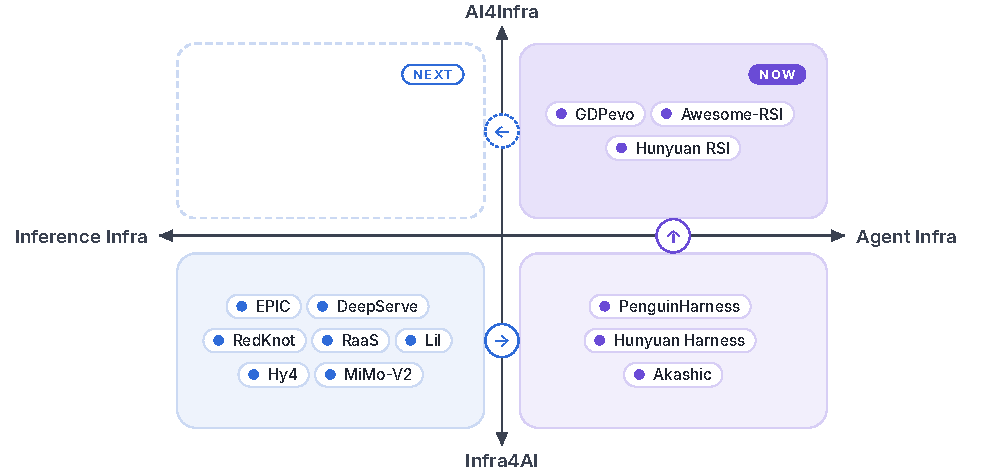
\includegraphics[width=0.9\textwidth]{figures/research-map.pdf}
\end{center}
